\begin{problem}
Find the best approximation from the space of polynomials of degree at
most one to $f(x) = x^2 , x \in [0 , 1]$ in:
\begin{enumerate}
\item $\infty$-norm.
\item 1-norm.
\item 2-norm.
\end{enumerate}
\end{problem}

\begin{solution}
  \begin{enumerate}
  \item [{\bf $\infty$-norm: }]:
    $\frac{\partial (kx + m - x^2)}{\partial x} = 0$ gives a critical
    point at $x = \frac{k}{2}$. This means the only three points we
    have to worry about is $x = 0, k/2, 1$ as they are the only
    possible maxima. The maximum error will be the smallest when all
    three maxima are equal. We used this same reasoning in the
    argument for the position of the Chebyshev points.

    If we make this demand and set the difference between the
    approximation function and $x^2$ to be equal to $\gamma$ at these
    three points we get a system of equations containing three
    equations and three unknowns.
    \begin{align}
      k \times 0  + m  - 0^2  = -\gamma \label{eq:start}\\
      k \times \frac{k}{2}  + m - \left(\frac{k}{2}\right)^2  = \gamma
      \label{eq:middle}\\
      k \times 1  + m  - 1^2   = -\gamma \label{eq:end}
    \end{align}
    Equation \ref{eq:start} gives $m = - \gamma$ and equation
    \ref{eq:middle} $k = \sqrt{8\gamma}$. Inserting this into equation
    \ref{eq:end} gives $\gamma = \frac{1}{8}$. Thus we have that the
    best approximation to $x^2$ in the approximation set of linear
    functions using the $\infty$-norm is $x - \frac{1}{8}$.
    
  \item [{\bf 2-norm}]:
    \begin{figure}[!ht]
      \centering
      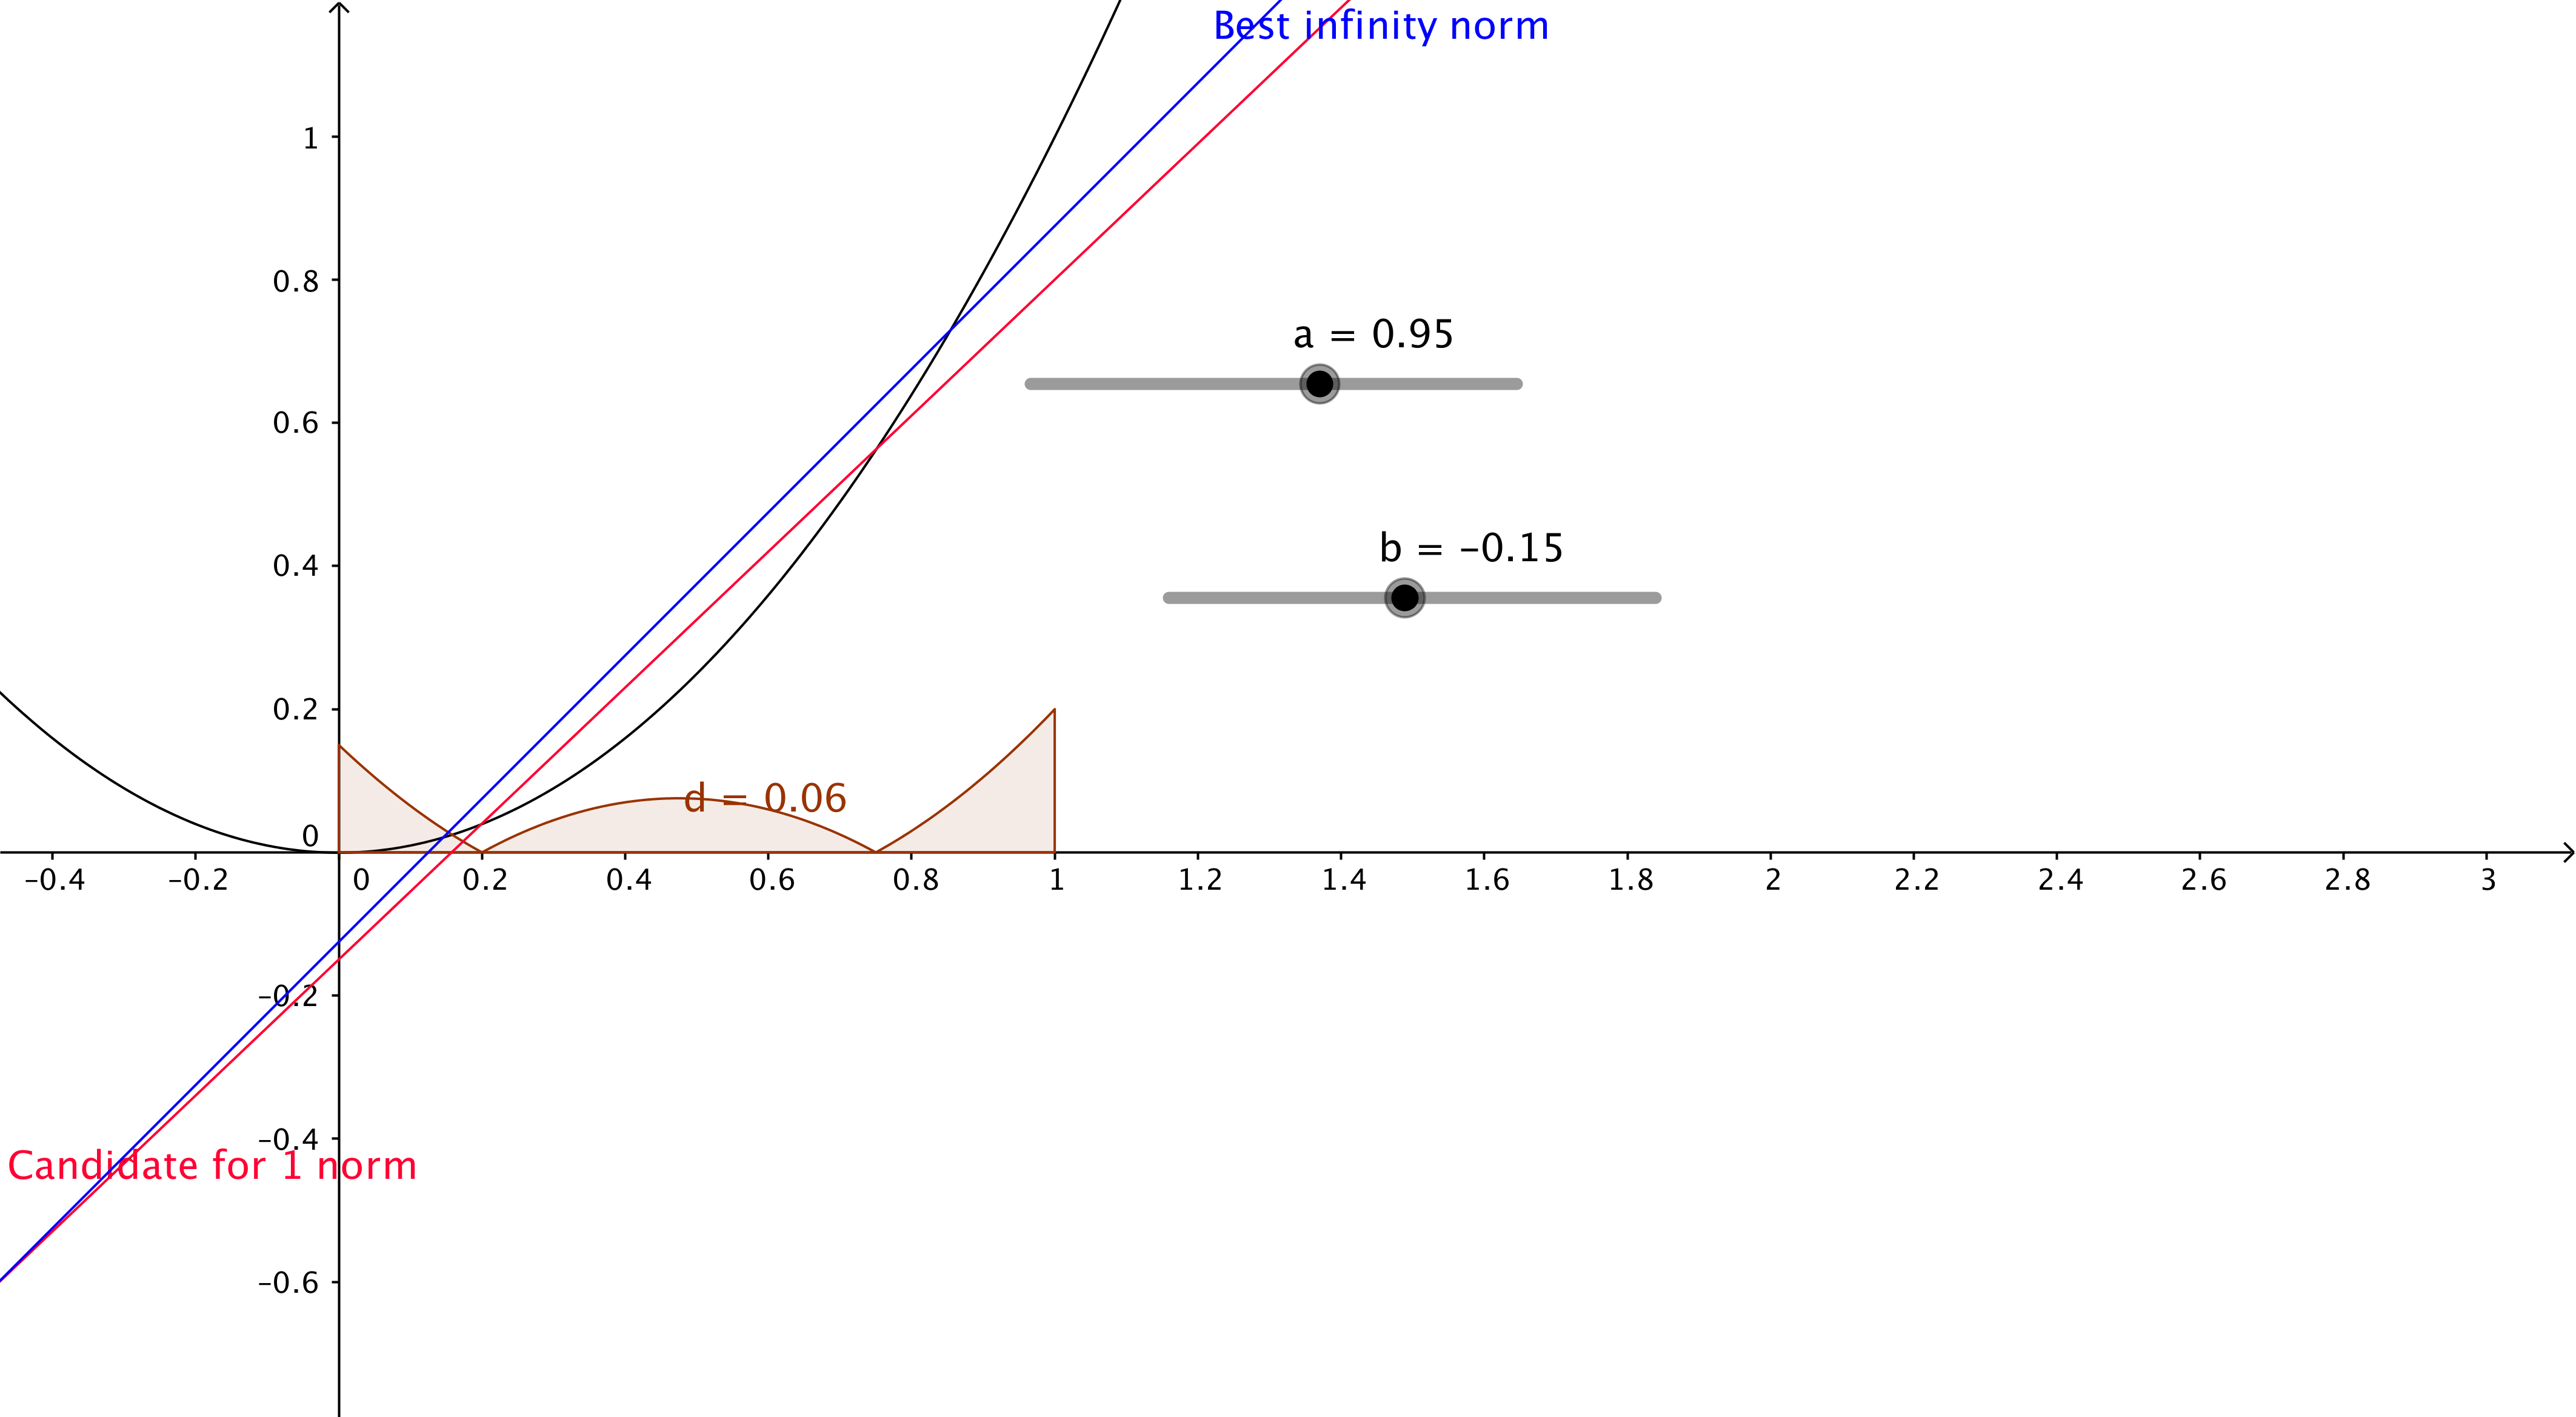
\includegraphics[scale = 0.2]{task7.png}
      \label{fig:task_7}
    \end{figure}

  \end{enumerate}
\end{solution}

 	

%%% Local Variables:
%%% TeX-master: "report.tex"
%%% End:
